% !TeX spellcheck = en_GB
% !TeX root = ../DistributedConsensus.tex
\chapter{Representing a History}\label{chap:representing-a-history}
	This chapter defines the representation of a \textit{history}. Furthermore it examines why a local history of a single event is a strict total order and a history of a workflow is a strict partial order.
	
    \section{Representation of an Execution}\label{sec:rep:exec}
    In order to find the order of execution in a workflow, one must first determine how to represent an execution. When an event executes it affects all of its relations. Furthermore since executions can happen multiple times, an execution also exists at a certain point in time, and so does every effect. This leads to the first definition of an \textbf{\textit{execution}}:
	
	\begin{definition}
		An \textbf{execution} of an event can be represented as a finite set of effects, and their timestamps. The set of effects are determined by the rules of the workflow.
	\end{definition}
	
	\noindent Timestamps based on system clocks in distributed systems are not always synchronized, as described in \autoref{subsec:orderingofevents}, and therefore Lamport's logical clocks can be used to determine the place in time of each effect. Since an effect both has an event which performs the effect and another event which gets affected, we say that each effect has a \textbf{\textit{counterpart}}\footnote{The idea of executions having effects on counterparts has been explored in \cite{debois2015safety}}:
	
	\begin{definition}
		In a given effect where two events A and B are part of the effect, event B is \textbf{\textit{counterpart}} of event A and event A is \textbf{\textit{counterpart}} of event B.
	\end{definition}
	
	\noindent To distinguish between the two events which takes part in the effect, it is necessary to use the IDs of both. Furthermore, to distinguish effects from each other an effect type is necessary. Since an execution can happen multiple times and therefore affect the same counterpart multiple times, the counterpart timestamp is also required to distinguish different effects on the counterpart from each other. To distinguish multiple executions from each other, an execution must have a start time and end time.
	
	\newpar For an event to know that something has happened, it is necessary to store it for later retrieval. This must be done for all effects on both sides of the effect.
	
	\newpar To make a common representation for what is stored, when an effect happens or the execution starts and finishes, the \textbf{\textit{action}} is introduced:
	
	\begin{definition}
		An \textit{\textbf{action}} consists of the ID of an event, the time stamp of the action, the ID and timestamp of a counterpart if relevant, as well as the type of the action.
	\end{definition}
	
	\newpar	The type of an action is defined as an \textit{\textbf{action type}}:
	
	\begin{definition}
        \label{def:actiontype}
		An \textit{\textbf{action type}} can be one of the following:
		\begin{multicols}{3}
			\begin{enumerate}
	            \item Checks condition\label{actiontype:checkscondition}
				\item Checked condition by\label{actiontype:checkedconditionby}
				\item Excludes\label{actiontype:excludes}
				\item Excluded by\label{actiontype:excludedby}
				\item Includes\label{actiontype:includes}
				\item Included by\label{actiontype:includedby}
				\item Sets pending\label{actiontype:setspending}
				\item Set pending by\label{actiontype:setpendingby}
				\item Execute start
				\item Execute finish
			\end{enumerate}
		\end{multicols}
	\end{definition}
	
	\newpar The action types 1 through 8 are related to the functionality of DCR graphs, i.e. \textit{Includes} is an action that happens when an event $A$ includes event $B$, similarly \textit{Included by} is an action that happens on event $B$ when event $A$ includes it. Action types 9 and 10 happen when an event starts executing and finishes executing.
    
    \newpar	Actions can form pairs according to their action types. Action types 1 through 8 in \autoref{def:actiontype} represent the types of the two sides of the effect.
	
	\begin{itemize}
		\item \textit{Outgoing action types} are action types \ref{actiontype:checkscondition}, \ref{actiontype:excludes}, \ref{actiontype:includes}, and \ref{actiontype:setspending}.
		\item \textit{Incoming action types} are action types \ref{actiontype:checkedconditionby}, \ref{actiontype:excludedby}, \ref{actiontype:includedby}, and \ref{actiontype:setpendingby}. 
	\end{itemize}
    
    \noindent For readability an \textit{outgoing action} is an action with an outgoing action type. In the same fashion an \textit{incoming action} is an action with an incoming action type.
    
    \newpar In this report we will use the following illustration types for signifying different entities:
    
    \begin{figure}[H]
		\centering
		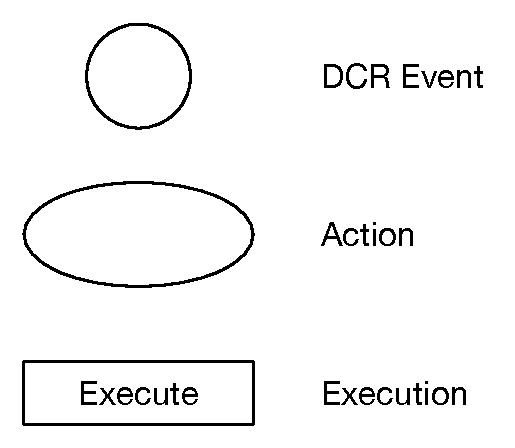
\includegraphics[height=0.20\textheight]{3local/images/legend.pdf}
		\caption{A legend showing what the different figures mean in the following sections.}
		\label{fig:representing:legend}
	\end{figure}
    
    
    \newpar An execution contains all the actions that was created as the result of the execution of an event, as illustrated in \autoref{fig:representing:execution-blobs}.
    
    \begin{figure}[H]
		\centering
		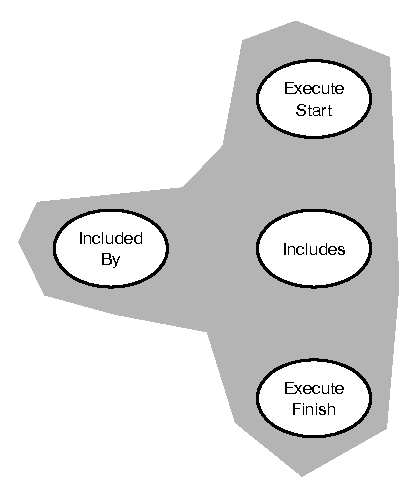
\includegraphics[height=0.35\textheight]{3local/images/execution-blobs.pdf}
		\caption{Actions that are part of an execution.}
		\label{fig:representing:execution-blobs}
	\end{figure}
    
	\noindent With these new informations the definition of a representation of an \textbf{\textit{exeuction}} can be revised to:
	
	\begin{definition}
		An \textbf{execution} of an event can be represented as a finite set of actions, which represents the effects that happened in the execution including two actions with action types \textbf{Execute start} and \textbf{Execute finish}, respectively.
		\label{def:execution}
	\end{definition}
	
    \noindent The ingoing actions of an execution will be stored at the counterpart which is not always the same event, as the one executing. This situation can be seen on \autoref{fig:representing:execution}.
    
    \begin{figure}[H]
		\centering
		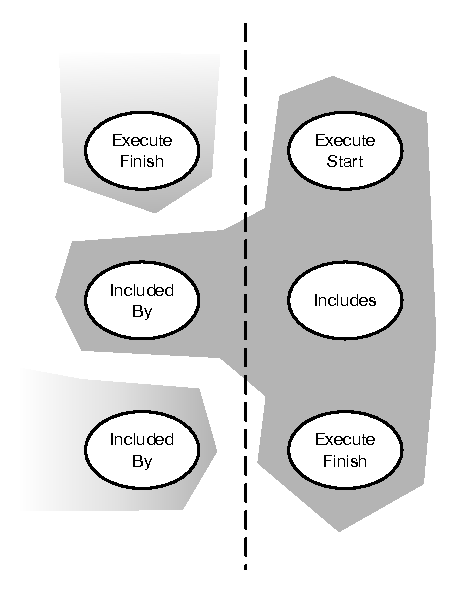
\includegraphics[height=0.35\textheight]{3local/images/execution.pdf}
		\caption{Actions that are part of an execution where an ingoing action is stored on another event.}
		\label{fig:representing:execution}
	\end{figure}

    \section{Representation of a History}\label{sec:rep:hist}
	Now that a representation of an execution and its actions has been defined, it is necessary to find a way to connect and order these actions.
    
    \newpar When looking solely at the actions of a single event, we can compare each action with any other action and see which happened first by comparing their timestamps. For an action to be part of an execution, it has to happen after an \textit{Execute start} and before an \textit{Execute finish}. Due to the requirement of DCR graphs that executions in an implementation must happen in a serially equivalent manner, all actions in execution $A$ must either happen before or after all actions in execution $B$ if the two executions are executions of the same event. Therefore, executions and their actions happening on the same event are in  \textit{strict total order}. Recall that Lamport states that it is not always possible to establish a strict total order of events in a distributed system, as described in \autoref{subsec:orderingofevents}. Therefore it is necessary to describe an invariant for executions of multiple events in a workflow:
	
	\begin{invariant}
		\begin{align*}
			(\exists{x\in E_A, y\in E_B}(x\rightarrow y) &\implies \forall{x\in E_A, y\in E_B}(y\not\rightarrow x))\\
			&\land \\
			\lnot(\exists{x\in E_A, y\in E_B}(x \rightarrow y)) &\implies \forall{x\in E_A, y\in E_B}(x\not\rightarrow y\land y\not\rightarrow x)
		\end{align*}
		\caption{Invariant for the actions of executions in histories}
		\label{inv:historyinvariant}
	\end{invariant}
	
	\newpar
	Invariant \ref{inv:historyinvariant} reads, if there exists an action, \textit{x}, in execution \textit{A}, and another action, \textit{y}, in execution \textit{B}, such that \textit{x} happens before \textit{y}, then for all actions \textit{x} in \textit{A} and all actions \textit{y} in \textit{B}, \textit{y} must not happen before \textit{x}. Otherwise there are no happens before relations between actions in \textit{A} and actions in \textit{B}.
    
	\newpar One can easily argue that a strict partial order fits ordering of actions because:
	\begin{enumerate}
		\item An action $A$ cannot happen before itself, therefore the order must be \textit{irreflexive}.
		\item Actions $A$ and $B$ cannot both be happening before and after each other, therefore the order must be \textit{anti-symmetric}.
		\item If action $A$ happened before action $B$ and $B$ happened before $C$ then $A$ happened before $C$ and the order must therefore be \textit{transitive}.
		\item Actions can in distributed systems be concurrent and the order can therefore not be \textit{total}.
	\end{enumerate}
	
	\newpar This leads to the following definition of \textbf{\textit{history}}:
	
	\begin{definition}
		A \textit{\textbf{history}} is a strict partial order of actions.
	\end{definition}
	
    \noindent A \textit{global history} is the strict partial order of the actions of all events in the workflow. A \textit{local history} is a strict total order of the actions that have happened on a single event.
    
    \newpar Since a finite strict partial order can be represented as a directed acyclic graph, the history can therefore also be represented as such, where actions are nodes and the order in which the actions have happened is represented as edges.

	
%	\begin{figure}
%		\centering
%		\import{3local/images/}{singleexecution.pdf_tex}
%		\caption{History representation of a single execution of the Event \texttt{ReadGasMeter}.}
%		\label{fig:local:readgasmeterhistory}
%	\end{figure}

%	\newpar When creating a history from the local database, the actions are added as nodes in the history, and since the ordering is total we can add edges between consecutive actions. An example of a local history is shown in \autoref{fig:local:readgasmeterhistory}.
	
	
%	\newpar In the implementation, we have created two types representing an action. One, the \texttt{ActionModel} is used for storage in the ORM Entity Framework.\footnote{Object-Relational Mapping, used for mapping between objects in an object-oriented paradigm and relations in a relational database.}\footnote{\url{https://msdn.microsoft.com/en-us/data/ef.aspx}} As this mapping is set up in a C\# library, this had to be a C\# class as well. The \texttt{ActionModel} uses the enum \texttt{ActionType} to denote the action type.
%	
%	The other type is created in the F\# module \texttt{HistoryConsensus} that contains most of the program described throughout this report. The \texttt{ActionType} in this module is a discriminated union, where each case represents a single type.\footnote{\url{https://msdn.microsoft.com/en-us/library/dd233226.aspx}}
%	In this module the type \texttt{ActionId} is defined as a tuple of an event ID and a local timestamp. The \texttt{Action} is then defined as a record  with two \texttt{ActionId}s, a local and a counterpart, as well as an \texttt{ActionType}.
%	
%	The \texttt{History} is implemented as a record with a single label called \texttt{Nodes}, containing a \texttt{Map} mapping from \texttt{ActionId} to the \texttt{Action} itself.
%	
%	\newpar As everything is handled locally at the event, no messages are passed between computers, other than the initial request for the local history, as well as the response. Retrieval of data from the database, as well as building the totally ordered history, takes time linear in the number of actions for that event, since the database is sorted and each event is accessed and used one at a time only once.
%	
%	\newpar In the case where a single event creates history, the event contacted has to be trusted as not being malicious. If the event cannot be trusted as behaving correctly, there are no guarantees that the history is correct, as it is the only source of its local history. Handling malicious nodes will be discussed further in the following chapters.
